\documentclass[12pt, a4paper]{article}
\usepackage[utf8]{inputenc}
\usepackage[russian]{babel}
\usepackage[T2A]{fontenc}
\usepackage{amsfonts}
\usepackage{amsmath}
\usepackage{indentfirst}
\usepackage{amsthm}
\usepackage{algorithm,algpseudocode}
\usepackage{caption}
\usepackage[labelfont=bf,textfont=normalfont,singlelinecheck=off,justification=raggedright]{subcaption}
\usepackage[hidelinks]{hyperref}
\DeclareMathOperator*{\minn}{min}
\DeclareMathOperator*{\argmin}{argmin}
\newtheorem{theorem}{Theorem}[section]
\newtheorem{state}{Утверждение}[section]
\newtheorem{lemma}{Лемма}[section]
\newtheorem{corollary}{Следствие}[section]


\usepackage[left=2cm,right=1.5cm,top=2cm,bottom=2cm]{geometry}
\linespread{1.25}

\usepackage{graphicx}
\graphicspath{{pictures/}}
\DeclareGraphicsExtensions{.pdf,.png,.jpg}

\begin{document}
\pagestyle{empty}

\begin{center}
	ФЕДЕРАЛЬНОЕ ГОСУДАРСТВЕННОЕ БЮДЖЕТНОЕ ОБРАЗОВАТЕЛЬНОЕ\\
	УЧРЕЖДЕНИЕ ВЫСШЕГО ОБРАЗОВАНИЯ\\
	<<МОСКОВСКИЙ ГОСУДАРСТВЕННЫЙ УНИВЕРСИТЕТ\\
	имени М.\,В.~ЛОМОНОСОВА>>
\end{center}
\vspace{4pt}
\begin{center}
	МЕХАНИКО-МАТЕМАТИЧЕСКИЙ ФАКУЛЬТЕТ
\end{center}
\vspace{4pt}
\begin{center}
	КАФЕДРА ВЫЧИСЛИТЕЛЬНОЙ МАТЕМАТИКИ
\end{center}
\vspace{1cm}
\begin{center}
	ВЫПУСКНАЯ КВАЛИФИКАЦИОННАЯ РАБОТА\\
	специалиста
\end{center}

\begin{center}
	\textbf{ОПТИМИЗАЦИЯ ТРАНСПОРТНОГО ПОТОКА \\
		    ПРИ ЗАДАННЫХ ПУНКТАХ ОТПРАВЛЕНИЯ И НАЗНАЧЕНИЯ \\
		    ВСЕХ УЧАСТНИКОВ ДВИЖЕНИЯ}
\end{center}
\vspace{1cm}
\begin{center}
	\begin{tabular}{p{9cm} l}
		& Выполнил студент $610$ группы\\
		& Пехтерев Станислав Игоревич\\
		& $\underline{\phantom{\int\limits_a^bf(x)dx=F(b)-F(a)}}$\\
		& подпись студента\\
		 $\phantom{C_n^k=C_n^{n-k}}$\\
		& Научный руководитель:\\
		& доктор физико-математических наук \\
		& Васенин Валерий Александрович\\
		& $\underline{\phantom{\int\limits_a^bf(x)dx=F(b)-F(a)}}$\\
		& подпись научного руководителя\\
		& $\phantom{C_n^k=C_n^{n-k}}$\\
		& кандидат физико-математических наук \\
		& Афонин Сергей Александрович\\
		& $\underline{\phantom{\int\limits_a^bf(x)dx=F(b)-F(a)}}$\\
		& подпись научного руководителя\\
	\end{tabular}
\end{center}
\vspace{1cm}
\begin{center}
	Москва\\
	$2022$
\end{center}

\newpage
\pagestyle{plain}
\tableofcontents{}
\newpage	

\addcontentsline{toc}{section}{Введение}
\section*{Введение}
Данная дипломная работа посвящена одной из задач математического моделировнаия транспортных потоков. А именно нас интересует построение оптимальных путей при заданных пунктах начала и конца всех участников движения на ориентированном графе в предположении, что участники следуют нашим рекомендациям. Участники могут оказывать влияние друг на друга, и что хорошо для одного, может критически отразиться на движении другого. Такая модель взаимодействия хорошо описывается некооперативной игрой, в процессе которой они не могут формировать коалиции и координировать свои действия. Однако наша задача --- скооперировать всех участников движения с помощью некоторой качественной оценки всевозможных комбинаций путей. Выбор такой оценки достаточно широк и неоднозначен и зависит от преследуемых целей. Они могут быть заданы приоритетами участников движения. Например, целью может быть обеспечение свободного передвижения служб спасения или кортежа, а может быть уменьшение общего времени движения участников.

Говоря об актуальности задачи, достаточно сказать, что на данный момент существует множество научных журналов\footnote{Перечень научных журналов: \textit{Transportation Research: Part B},
	\textit{Physical Review E}, \textit{Review of modern physics}, \textit{Transportation Science.}}, в которых регулярно публикуются статьи на транспортную тематику. Также известное немецкое издательство \textit{Springer} публикует труды ученых, представленных на конференции по математическому моделированию транспортных потоков ``\textit{Traffic and granular flow}'', которая проводится с периодичностью в 2 года.

На сегодняшний день предложено множество математических моделей, позволяющих исследовать движения участников, однако они имеют свои недостатки. Так, например, в учебном пособии А.\,Е.~Гасникова~\cite{book} изложены модели, описывающие плотный статический поток машин, передвигающихся из множества точек истока во множество точек сток. Такой подход является корректным, только если в каждый момент времени на участке некоторого пути можно задать постоянную плотность машин --- количество машин на единицу длины. Также в учебном пособии отдельное место занимает применение теории гидродинамики к описанию движения транспортных потоков. Их представляют как потоки сжимаемой жидкости, описываемые законом сохранения количества автомобилей. В отличие от предыдущей модели, этот подход подразумевает возможность исследования нестатического потока, но не позволяет отслеживать движения участников на путях.
%Минусы моделей: да, участники взаимодействуют, но не для каждого взаимодействия их можно описать в таких моделях. 

Наш подход заключается в задании некоторой модели взаимодействия участников, с помощью которой можно полностью промоделировать движение каждого из них. 
Основа модели --- ограничения на скорости и законы их изменения при взаимодействии участников друг с другом. Такой подход отличается индивидуализуацией участников движения --- их количественные характеристики могут быть исследованы по отдельности. Заданная нами модель взаимодействия участников способна описать естественное движение автомобилей, что позволяет исследовать влияние добавления или расширения дорог на количество и длины пробок.

Общая постановка задачи, описанная в первом разделе, основана только на функции затрат, 
однако во втором разделе будет показана возможность задания некоторой модели движения, описывающей взаимодействие участников.
В том же разделе будут разработаны и исследованы некоторые модели движения участников, будет предложена классификация этих моделей. Среди них мы выделим класс, для которого доказана возможность сведения задачи оптимизации к задаче смешанного целочисленного линейного программирования. В третьем разделе, руководствуясь принципами в теории транспортного равновесия, мы попробуем решить задачу построения оптимальных маршрутов путем поиска таких равновесий. В завершение будут рассмотрены практические интерпретации задачи и описаны результаты их исследования.

\newpage
\section{Постановка задачи}

Для начала сформулируем задачу оптимизации транспортного потока в общей форме.
В разделе \ref{sec:concrete} мы конкретизируем постановку задачи, задав участникам некоторую модель движения.

\subsection{Общая постановка задачи}

\textit {Дорожной сетью} назовем тройку $G = (V, E, l)$, где $(V, E)$ --- ориентированный граф с длинами ребер $l: E \rightarrow \mathbb{R}_{>0} $.  Предположим, что имеется $n$ участников с заданными точками отправления $A_i \in V$ и прибытия $B_i \in V$. Пусть множество $P_i$ есть множество всех простых путей из $A_i$ в $B_i$. Элемент декартового произведения ${P = \prod \limits_{i = 1} ^ n P_i}$ назовем \textit{комбинацией путей}. Пусть известно, что при комбинации путей участников $\textbf{p} = \left(p_1, \ldots, p_n\right)\in P$ $i$-ый участник затрачивает $T_i(\textbf{p}) \in \mathbb{R}_{\ge 0}$ времени на свой путь. 
Функции $T_i$ назовем \textit{функциями временных затрат} участника $i$.
\textit{Некооперативным прокладыванием пути} в дорожной сети $G$ назовем пятерку $F = (n, G, \{A_i\}_{i = 1}^{n}, \{B_i\}_{i = 1}^{n}, \{T_i\}_{i = 1}^{n})$. Некооперативное прокладывание пути предполагает, что каждый участник стремится сократить собственные временные затраты выбором пути $p_i$, несмотря на временные затраты других участников \cite{teor_igri}. 
Для того, чтобы скооперировать участников, введем некоторую функцию $\Phi (\textbf{p}) = \phi (T_1 (\textbf{p}), \ldots, T_n(\textbf{p}))$, определенную на множестве всех возможных комбинаций путей $P$ и отображающую его во множество действительных чисел. С помощью нее участники могут отслеживать, как влияет изменение их пути на общую картину движения. Такую функцию назовем \textit{функцией стоимости}.

Для заданных некооперативного прокладывания пути $F$ и функции стоимости $\Phi$ необходимо найти комбинацию путей $\textbf{p}^*$ такую, что функция стоимости на ней минимальна, то есть
\begin{equation}
	\label{eq:target_global_task_T} 
	\Phi (\textbf{p}^*) = \minn\limits_{ \textbf{p} \in P} \Phi (\textbf{p}).
\end{equation}

Комбинацию путей $\textbf{p}^*$ будем называть \textit {оптимальной}, а стоимость  $ \Phi (\textbf{p}^*)$ --- \textit{оптимальной стоимостью}.

Если нет каких-либо ограничений на функцию $\phi$, то решение задачи \eqref{eq:target_global_task_T} можно найти только перебором, поэтому будем рассматривать функции $\phi$ специального вида $$\phi(T_1, \ldots, T_n) = \sum\limits_{i = 1}^n \gamma_iT_i,$$ где $\gamma_i \in \mathbb{R}_{\ge 0}$ --- приоритет участника $i$. В данном работе мы рассматриваем случай, когда каждый участник имеет одинаковый приоритет, то есть 
\begin{equation}
\label{target_f}
\phi(T_1, \ldots, T_n) = \sum\limits_{i = 1}^nT_i.
\end{equation}
Заметим, что некоторые результаты в данной работе применимы для более широкого класса функций $\phi$. 

Пока не понятно, каким образом стоит задавать функции $T_i (\textbf{p})$ и как заложить в них взаимодействие участников. Далее постараемся описать общий принцип взаимодействия участников на основе задания некоторой модели движения и покажем, что такой принцип не ограничивает нас в выборе $T_i (\textbf{p})$.

\subsection{Постановка задачи в терминах модели движения}

\label{sec:concrete}
Будем считать, что временные затраты участника на выбранном пути состоят из временных затрат на каждом ребре этого пути:
$$T_i (\textbf{p}) = \sum \limits_{e \in p_i} \overline{\tau}_{e, i} (\textbf{p}), $$
где функции $\overline{\tau}_{e, i} (\textbf{p})$ --- временные затраты $i$-ого участника на ребре $e$ при комбинации путей $\textbf{p}$. 

%например затраты возрастают, когда кто-то еще проезжает по ребру

Для того, чтобы задать движение участника на пути, введем функции присутствия участника на ребре в момент времени $t$:
%%Будем рассматривать те некооперативные прокладывания пути, в которых
% существует движение каждого участника для каждой комбинации путей $\textbf{p}$, то есть 
%в каждый момент времени $t \in \mathbb{R}$ известно положение участника на пути. Таким образом, будем считать, что для каждой комбинации путей $\textbf{p}$ и времени $t$ известно присутствует ли участник $i$ на ребре $e$, то есть известны функции
$$
\theta_{e, i} (\textbf{p}, t) =
\begin{cases}
	1, & \text{если }  i\text{-ый участник движется по ребру $e$ в момент времени $t$,}  \\
	0, & \text{иначе},
\end{cases}
$$
где $\sum\limits_{e \in E} \theta_{e, i} (\textbf{p}, t)$ принимает значение $1$, пока $i$~-ый участник не посетит свою точку назначения $B_i$. Пусть достижение конца пути $p_i$ наступает в момент $T_i(\textbf{p})$, после чего $\sum\limits_{e \in E} \theta_{e, i} (\textbf{p}, t)$ принимает значение $0$. Получаем, что
\begin{equation}
	\label{eq:T_i_by_theta}
	T_i(\textbf{p}) = \sum \limits_{e \in p_i} \int\limits_{0}^{\infty} \theta_{e, i} (\textbf{p}, t) dt, \; \forall \Delta t > 0.
\end{equation}

Будем считать, что движение каждого учаcтника является непрерывным и однонаправленным в дорожной сети $G$. Другими словами, участник не может резко повляться и исчезать на несмежных ребрах, а также находиться на уже пройденных ребрах. Таким образом, функции $\theta_{e, i} (\textbf{p}, t)$ являются индикаторами некоторых временных отрезков $[t_{e, i}^{in} (\textbf{p}), t_{e, i}^{out} (\textbf{p})]$, которые описывают однонаправленное движение:
\begin{equation}
	\label{eq:restr_t}
	\begin{cases}
		t_{e, i}^{in}(\textbf{p}), t_{e, i}^{out}(\textbf{p}) \in \mathbb{R}_+,  & i = 1, \dots, n, \text{ } e \in E, \\
		t_{e, i}^{in}(\textbf{p}) \le t_{e, i}^{out}(\textbf{p}), & i = 1, \dots, n, \text{ } e \in p_i,  \\
		t_{e, i}^{in}(\textbf{p}) = t_{e, i}^{out}(\textbf{p}) = 0, & i = 1, \dots, n, \text{ } e \notin p_i, \\
		t_{e_1, i}^{in} (\textbf{p}) = t_{e_2, i}^{out} (\textbf{p}), & i = 1, \dots, n, \text{ } e_1, e_2 \in p_i, \; \exists A, B, C \in V: e_1 = (A, B), e_2 = (B, C)\\
		t_{e, i}^{in} (\textbf{p}) = 0, & i = 1, \dots, n, \text{ } e = (A_i, X), \; X \in V.
	\end{cases}
\end{equation}

Заметим, что выбор таких отрезков пока неоднозначен. Далее считаем, что для каждого ребра $e$, участника $i$ и комбинации путей $\textbf{p}$ каким-то образом выбраны некоторые величины $t_{e, i}^{in}(\textbf{p}), \: t_{e, i}^{out}(\textbf{p})$, удовлетворяющие ограничениям \eqref{eq:restr_t}. Тогда функция временных затрат \eqref{eq:T_i_by_theta} $i$-ого участника примет вид
\begin{equation}
	\label{eq:T_i_by_t}
	T_i(\textbf{p}) = \sum \limits_{e \in E} t_{e, i}^{out}(\textbf{p}) - t_{e, i}^{in}(\textbf{p}).
\end{equation}

Функция стоимости в этом случае равна 
\begin{equation}
	\label{eq:target_func}
	\Phi(\textbf{p}) =\sum \limits_{i = 1}^n \sum \limits_{e \in E} t_{e, i}^{out}(\textbf{p}) - t_{e, i}^{in}(\textbf{p}).
\end{equation}

Считаем, что временные затраты участника $i$ на ребре $e$ ограничены некоторыми положительными константами $\overline{\tau}_{e, i}^{min}, \: \overline{\tau}_{e, i}^{max}$:
\begin{equation}
	\label{eq:add_restr}
		0 < \overline{\tau}_{e, i}^{min} \le t_{e, i}^{out}(\textbf{p}) - t_{e, i}^{in}(\textbf{p}) \le \overline{\tau}_{e, i}^{max}, \; e \in p_i,\, \; i = 1, \dots, n.
\end{equation}

Заметим, что задача оптимизации целевой функции \eqref{eq:target_func} с ограничениями \eqref{eq:restr_t}, \eqref{eq:add_restr} ставится в терминах задачи смешанного целочисленного линейного программирования \cite{min_ip_tsp} с булевыми переменными $I_{e, i}$ и вещественными переменными $t_{e, i}^{in}, \: t_{e, i}^{out}$. Для участника $i$ первые отвечают факту проезда по ребру $e$, вторые --- моментам прохождения этого ребра. Однако в данных ограничениях решение уже есть --- участник $i$ передвигается по кратчайшему пути в дорожной сети $G$ с весами $\overline{\tau}_{e, i}^{min}$. Тривиальность решения связана с тем, что в данной задаче оптимизации отсутствуют влияния участников друг на друга. Для того, чтобы учесть это влияние, для каждого участника $i$ введем микроскопическую характеристику движения $v_i(\textbf{p}, t)$ ~--- положительную, ограниченную функцию, описывающую скорость участника.
Тогда имеет место следующее ограничение
\begin{equation}
	\label{eq:velocity_eq_by_theta}
	\int\limits_{0}^{\infty} \theta_{e, i} (\textbf{p}, t) v_i(\textbf{p}, t) dt = l_e, e \in p_i, i = 1, \dots, n,
\end{equation}
или
\begin{equation}
	\label{eq:velocity_eq_by_t}
	\int\limits_{t_{e, i}^{in}(\textbf{p})}^{t_{e, i}^{out}(\textbf{p})} v_i(\textbf{p}, t) dt = l_e, e \in p_i, i = 1, \dots, n.
\end{equation}

Будем говорить, что уравнения \eqref{eq:velocity_eq_by_t} задают \textit{движения участников}, а функции $v_i(\textbf{p}, t)$ назовем \textit{моделью движения}. Будем считать, что функции $v_i$ ограничены некоторыми положительными константами. Обозначим верхние и нижне грани этих функци  $v_i^{max} > 0$ и $v_i^{min} > 0$ сответственно. Без ограничения общности считаем, что $\overline{\tau}_{e, i}^{min}, \: \overline{\tau}_{e, i}^{max}$ вычисляются в самом быстром и самом медленном вариантах передвижения по ребру $e$ участником $i$, а именно
\begin{equation}
	\label{eq:restr_add_concrete}
	\overline{\tau}_{e, i}^{min} = \frac{l_e}{v_i^{max}}, \; \overline{\tau}_{e, i}^{max} = \frac{l_e}{v_i^{min}}.
\end{equation}

Заметим, что величины $t_{e, i}^{in}(\textbf{p}), \: t_{e, i}^{out}(\textbf{p}) \in \mathbb{R}_+$ --- произвольные вещественные величины, которые удовлетворяют ограничениям \eqref{eq:restr_t}, \eqref{eq:add_restr}, \eqref{eq:velocity_eq_by_t}, \eqref{eq:restr_add_concrete}.

\begin{state}
\label{state:modeling}
Пусть задана дорожная сеть $G$, модель движения $v_i(\textbf{p}, t)$, и для каждого ребра $e$, участника $i$ и комбинации путей $\textbf{p}$ задано множество величин $t_{e, i}^{in}(\textbf{p}), \: t_{e, i}^{out}(\textbf{p}) \in \mathbb{R}_+$, для которых выполняются ограничения \eqref{eq:restr_t}, \eqref{eq:add_restr}, \eqref{eq:velocity_eq_by_t}, \eqref{eq:restr_add_concrete}. Тогда $t_{e, i}^{out}(\textbf{p})$ и $t_{e, i}^{in}(\textbf{p})$, $e \in p_i$ есть функции от комбинации путей $\textbf{p} \in P$.
\end{state}
\begin{proof}
Зафиксируем некоторую комбинацию путей $\textbf{p}$. Опишем алгоритм поиска значений $t_{e, i}^{out}(\textbf{p})$ и $t_{e, i}^{in}(\textbf{p})$ и покажем его корректность.

\begin{algorithm}[H]
	\caption{Моделирование движения участников}
	\label{alg:modeling}
	{\bf {Input:}} количество участников $n$, дорожная сеть $G$, комбинация путей $\textbf{p}$ сети $G$\\
	{\bf {Output:}} $t_{e, i}^{out}(\textbf{p})$, $t_{e, i}^{in}(\textbf{p})$, $e \in p_i, i = 1, \ldots, n$\\
	{\bf {Data:}} текущее время $t$, текущее ребро $e_i$ и часть пройденного ребра $x_i$ участника $i$
	\begin{algorithmic}[1]
		\State $t = 0$
		\For{$i = 1, \ldots, n$}
		\State $e_i \gets$ { первое ребро пути $p_i$}
		\State $x_i \gets 0$
		\State $t_{e_i, i}^{in}(\textbf{p}) \gets 0$ 
		\EndFor
		\While{$\exists j: j \text { --- не достиг } B_j$}
		\State $\tau^* \gets \argmin\{ \tau \in \mathbb{R}: \tau > t, \; \int\limits_{t}^{\tau} v_i(\textbf{p}, t) dt = (1 - x_i) l_{e_i}, \; i \text { --- не достиг } B_i  \}_{i = 1}^n$
		\For{$i = 1, \ldots, n$ \textbf{and} $i \text { --- не достиг } B_i$ }
		\State $x_i \gets x_i + \frac{1}{l_{e_i}} \int\limits_{t}^{\tau^*} v_i(\textbf{p}, t) dt$
			\If{$x_i = 1$ \textbf{and} $e_i$ - не последнее ребро пути $p_i$ }
				\State $x_i \gets 0$
				\State $t_{e_i, i}^{out}(\textbf{p}) \gets \tau^*$ 
				\State $e_i \gets$ следующее ребро за $e_i$ в пути $p_i$
				\State $t_{e_i, i}^{in}(\textbf{p}) \gets \tau^*$ 
			\EndIf
		\EndFor
		\State $t \gets \tau^*$
		\EndWhile
	\end{algorithmic}
\end{algorithm}


Будем называть данный алгоритм \textit{моделированием движения}.

\textit{Корректность}. Для доказательства корректности алгоритма достаточно доказать корректность шага 8 и достижимость шага 11. Это следует из того, что для каждого участника $i$ функция скорости ограничена снизу некоторой константой $v_i^{max}$. Алгоритм сойдется, поскольку пути $p_i$ конечны.

\end{proof}
%Заметим, что сложность моделирования во многом зависит от количества способов взаимодействия участников.
Используя это утверждение, можем ввести следующее понятие:

\textit{Некооперативным передвижением} в дорожной сети $G$ в модели движения $v_i(\textbf{p}, t)$ назовем такое некооперативное прокладывание пути \\$F = \left(n, G, \{A_i\}_{i = 1}^{n}, \{B_i\}_{i = 1}^{n}, \left\{\sum\limits_{e \in p_i} t_{e, i}^{out}(\textbf{p}) - t_{e, i}^{in}(\textbf{p})\right\}_{i = 1}^{n}\right)$, где функции $t_{e, i}^{in}(\textbf{p}), \: t_{e, i}^{out}(\textbf{p})$ получены путем моделирования движения с моделью движения $v_i(\textbf{p}, t)$.
Значит, постановка задачи в терминах модели движения следующая:

Пусть задано некооперативное передвижение в дорожной сети $G$ в модели движения $v_i(\textbf{p}, t)$.
Требуется найти комбинацию путей $\textbf{p}$ такую, что функция 

\begin{equation}
\label{eq:target_task_end}
\Phi(\textbf{p}) =\sum \limits_{i = 1}^n \sum \limits_{e \in E} t_{e, i}^{out}(\textbf{p}) - t_{e, i}^{in}(\textbf{p})
\end{equation}
минимальна.


\newpage
\section{Модели движения}

\label{sec:models}
Часто для описания движения функции $v_i(\textbf{p}, t)$ задают на основе некоторых правил движения. Именно в этих правилах заложено взаимодействие участников. Например,  
\begin{enumerate}
	\item Тормозим, если впереди идущий слишком близко к нам.
	\item Ускоряемся, если впереди идущий достаточно далеко от нас.
	\item Не превышаем некоторую скорость.
	\item Тормозим перед поворотом.
\end{enumerate}
Значения функции $v_i(\textbf{p}, t)$ могут быть вычислены применением правил движения в момент моделирования (см. алгоритм \ref{alg:modeling}).

Оказывается, что для любого некооперативного прокладывания пути существует, по крайней мере, одна модель движения, описывающая некооперативное прокладывание пути.

\begin{state}
	\label{state:eqv}
	Пусть заданы некоторое некооперативное прокладывание пути $F$. Тогда можно задать такую модель движения $v_i(\textbf{p}, t)$, что затраченное время на передвижение $i$-ым участником при комбинации путей $\textbf{p}$ совпадает с его временными затратами при моделировании, то есть выполняется \eqref{eq:T_i_by_t}.
	
\end{state}

\begin{proof}
Рассмотрим модель движения с постоянными скоростями  
$$v_i(\textbf{p}, t) = \overline{v}_i(\textbf{p}) = \frac{T_i (\textbf{p})}{\sum \limits_{e \in p_i} l_e}.$$

Промоделировав движение с такими скоростями, получим \eqref{eq:T_i_by_t}.
\end{proof}

Таким образом, введя модель движения мы не ограничиваем себя в выборе функций $T_i (\textbf{p})$.

Очевидно, что решение задачи перебором не является практичным --- оно сводится к перебору всех комбинаций путей $\textbf{p} \in P$. Так, например, количество таких комбинаций в полном графе составляет $$|P| = \left(\sum\limits_{k = 1}^{|V| - 2} k!\right)^n,$$ перебрать которые в условиях реальных данных вычислительно сложно.
Однако в случае, когда условие \eqref{eq:velocity_eq_by_t} можно описать в терминах задачи удовлетворения ограничений \cite{UO}, задача оптимизации \eqref{eq:target_task_end} может быть описана в терминах смешанного целочисленного линейного программирования и, как следствие, может быть решена стандартным решателем \footnote{\url{https://www.gurobi.com}}. Оказывается, можно выделить целый класс таких моделей движения, для которых это возможно.

\subsection{Макроскопические модели}

Предположим, что скорость участника зависит от некоторой общей для участников величины. Например, от функции \textit{загруженности ребра}
$$ n_{e}(\textbf{p}, t) = \sum\limits_{i = 1}^n\theta_{e, i}(\textbf{p}, t),$$
значение которой в момент времени $t$ соответствует количеству участников на ребре $e$ при комбинации путей $\textbf{p}$. Предположим, скорость участника зависит только от загруженности ребра, на котором он находится в момент времени $t$, то есть существует ограниченная функция $v : \{0, 1, \dots, n\} \rightarrow \mathbb{R}_{> 0}$ такая, что
\begin{equation}
	\label{eq:velocity_eq_macro}
	 v_i(\textbf{p}, t) = \sum \limits _{e \in E} \theta_{e, i} (\textbf{p}, t) v (n_e (\textbf{p}, t)), \; i = 1, \dots, n
\end{equation}

Такую модель движения в дальнейшем будем называть \textit{макроскопической}.
Например, естественно рассмотреть модель
\begin{equation}
\label{eq:best_macro}
v (n_e (\textbf{p}, t)) = \frac{v_{max}}{n_e (\textbf{p}, t)}. 
\end{equation}
В разделе \ref{sec:rovn} покажем, что при таком взаимодействии участников \eqref{eq:best_macro} в статическом некооперативном передвижении\footnote{Некооперативное передвижение называется статическим, если функция $n_e (\textbf{p}, t)$ не зависит от времени $t$.} верно, что для некооперативного равновесия $\widehat{\textbf{p}} \in P$ верна оценка
 $$ \frac{\Phi(\widehat{\textbf{p}})}{\Phi(\textbf{p}^*)} \le \frac{4}{3}.$$
 
В общем случае такая модель задается последовательностью значений  $\{v(k)\}_{k = 1}^n$.

\begin{lemma}
	\label{lemma:lt}
	Пусть даны вещественные переменные $a$, $b$ целочисленного программирования, и известно, что существует константа $M > 0$: $|a| < M$, $|b| < M$. Тогда можно добавить новую целочисленную переменную $\textbf{1} (\{a < b\}) \in \{0, 1\}$ такую, что
	\begin{equation*}
		\textbf{1} (\{a < b\}) = 
		\begin{cases}
			1,\, a < b,
			\\
			0,\, a \ge b.
		\end{cases}
	\end{equation*}

\end{lemma}

\begin{proof}
	Добавим в нашу задачу два неравенства:
	$$ 2M (\textbf{1} (\{a < b\}) - 1) < b - a \le 2M\textbf{1} (\{a < b\}) $$
	
	Очевидная проверка показывает, что неравенство выполняется для любых $a, b$.
	
	
\end{proof}

\begin{state}
	
	\label{state:lin_prog}
	
	Пусть модель движения $ v_i(\textbf{p}, t)$ макроскопическая. Тогда задача \eqref{eq:target_task_end} есть задача смешанного целочисленного линейного программирования.
\end{state}

\begin{proof}
	Докажем для случая $n = 2$. Для случаев $n \ge 2$ доказательство аналогичное.
	
	Пусть имеется задача смешанного целочисленного линейного программирования \eqref{eq:restr_t} с переменными $t_{e, i}^{in}, \: t_{e, i}^{out}, \: I_{e, i}, \; e \in E, \; i = 1, 2$. Преобразуем условие \eqref{eq:velocity_eq_by_t} к каноническому виду задачи удовлетворения ограничений. Для удобства обозначим обоих участников индексами $i, j \in \{1, 2\}$.
	
	$$\int\limits_{0}^{\infty} \theta_{e, i} (\textbf{p}, t) v_i(\textbf{p}, t)dt = \int\limits_{0}^{\infty} \theta_{e, i} (\textbf{p}, t) \sum \limits _{e^1 \in E} \theta_{e^1, i} (\textbf{p}, t) v (n_{e^1} (\textbf{p}, t)) dt = $$
	
	$$\int\limits_{0}^{\infty} \theta_{e, i} (\textbf{p}, t)  v (n_{e} (\textbf{p}, t)) dt = 
	  \int\limits_{ \substack{n_{e} (\textbf{p}, t) = 1}} \theta_{e, i} (\textbf{p}, t)  v (n_{e} (\textbf{p}, t)) dt \; +
	  \int\limits_{ \substack{n_{e} (\textbf{p}, t) = 2}} \theta_{e, i} (\textbf{p}, t)  v (n_{e} (\textbf{p}, t)) dt = $$
	
	$$\int\limits_{ \substack{\theta_{e, j} (\textbf{p}, t) = 0}} \theta_{e, i} (\textbf{p}, t)  v (1) dt \; +
	  \int\limits_{ \substack{\theta_{e, j} (\textbf{p}, t) = 1}} \theta_{e, i} (\textbf{p}, t)  v (2) dt = $$
	  
    $$\int\limits_{0}^{\infty} \theta_{e, i} (\textbf{p}, t)  v (1) dt \; - 
      \int\limits_{ \substack{\theta_{e, j} (\textbf{p}, t) = 1}} \theta_{e, i} (\textbf{p}, t)  v (1) dt \; +
	  \int\limits_{ \substack{\theta_{e, j} (\textbf{p}, t) = 1}} \theta_{e, i} (\textbf{p}, t)  v (2) dt = $$
	  
	$$v (1) \int\limits_{0}^{\infty} \theta_{e, i} (\textbf{p}, t) dt \; + \;
	  (v (2) - v(1)) \int\limits_{0}^{\infty} \theta_{e, i} (\textbf{p}, t) \theta_{e, j} (\textbf{p}, t) dt = $$
	  
    $$v (1) \overline{\tau}_{e, i} (\textbf{p}) \; + \;
    (v (2) - v(1)) \int\limits_{0}^{\infty} \theta_{e, i} (\textbf{p}, t) \theta_{e, j} (\textbf{p}, t) dt = l_e, \; e \in p_i$$
	  
	Неизвестный интеграл --- время совместного проезда участников на ребре $e$.
	  
	В переменных задачи смешанного целочисленного программирования получим:
	$$v(1) (t_{e, i}^{out} - t_{e, i}^{in}) + (v(2) - v(1)) (t_{e, ij}^{out} - t_{e, ij}^{in}) = l_e I_{e, i},$$
	где новые переменные $t_{e, ij}^{in}$, $t_{e, ij}^{out}$ отвечают началу и концу совместного проезда участников. Иначе говоря, $[t_{e, ij}^{in}, \: t_{e, ij}^{out}] = [t_{e, i}^{in}, \: t_{e, i}^{out}] \cap [t_{e, j}^{in}, \: t_{e, j}^{out}]$. Просуммировав по всем ребрам $e \in E$, получим
	$$v(1) \sum \limits _{e \in E} (t_{e, i}^{out} - t_{e, i}^{in}) = \sum \limits _{e \in E} l_e I_{e, i} - (v(2) - v(1)) \sum \limits _{e \in E} (t_{e, ij}^{out} - t_{e, ij}^{in}).$$
	Заметим, что левая часть представляет собой временные затраты участника $i$ с коэффициентом $v(1)$, поэтому задачу оптимизации можно переписать в виде
	$$ \frac{1}{v (1)} \sum\limits_{i = 1}^n \sum \limits _{e \in E} l_e I_{e, i} + \frac{v(1) - v(2)}{v (1)}  \sum\limits_{i = 1}^n \sum \limits _{e \in E} (t_{e, ij}^{out} - t_{e, ij}^{in}) \rightarrow \minn .$$
	
	Для завершения доказательства необходимо показать, что переменные $t_{e, ij}^{in}, \: t_{e, ij}^{out}$ описываются линейными ограничениями. Обозначим
	\begin{align*}
		& \Delta t = t_{e, ij}^{out} - t_{e, ij}^{in} \\
		& \Delta t_1 =  t_{e, i}^{out} - t_{e, i}^{in}  \\
		& \Delta t_2 =  t_{e, j}^{out} - t_{e, j}^{in} \\
		& \Delta t_3 =  t_{e, i}^{out} - t_{e, j}^{in} \\
		& \Delta t_4 =  t_{e, j}^{out} - t_{e, i}^{in}.
	\end{align*}
	Используя лемму \ref{lemma:lt} при $M = \max\limits_{e \in E, k = i, j} \overline{\tau}_{e, k}^{max}$, добавим в задачу новые переменные $\textbf{1} (\{ \Delta t_k > \Delta t_l\}), \; k \ne l, \; k, l \in \{1, 2, 3, 4\}$. Рассмотрим величину $T_{max} = |E|M$. В случае $v(1) \ge v(2)$ добавим в нашу задачу следующие неравенства: 
	\begin{align*}
	& \Delta t \ge 0, \\
	& \Delta t \ge \Delta t_k - T_{max} \sum \limits_{l \ne k} {\textbf{1} (\{ \Delta t_k > \Delta t_l\})}, \; k = 1, 2, 3, 4.
	\end{align*}
	В случае $v(1) < v(2)$ добавим те же ограничения с другим знаком неравенства. Тогда с учетом оптимизации переменная $\Delta t$ есть длина отрезка $[t_{e, ij}^{in}, \: t_{e, ij}^{out}]$. 
	
\end{proof}

\begin{corollary}
	\label{corollary:rel}

	Пусть модель движения $ v_i(\textbf{p}, t) = \sum \limits _{e \in E} \theta_{e, i} (\textbf{p}, t) v (n_e (\textbf{p}, t))$ макроскопическая и последовательность $v(n) > 0, \; \forall n \in \mathbb{Z}_+$ убывает. Предположим, что оптимальное время движения в модели c постоянной скоростью $v(1)$ есть $\widetilde{T}$. Тогда
	$$ \widetilde{T} \le T \le \frac {v(1)}{v(n)} \widetilde{T}.$$
	
\end{corollary}

\begin{proof}
	Докажем каждое неравенство по отдельности
	
	1. В модели, где все участники едут с постоянными скоростями, движение происходит по кратчайшим путям. Тогда временные затраты есть $\widetilde{T} = \frac{1}{v(1)} \sum \limits _{i = 1} ^ n \sum\limits_{e \in p_i} l_e$, где $p_i$ - кратчайшие пути.
	На тех же путях задается худший случай макроскопической модели --- все едут с минимальной скоростью, то есть $ T = \frac{1}{v(n)} \sum \limits _{i = 1} ^ n \sum\limits_{e \in p_i} l_e$. Тогда получим
	$$T \le  \frac{1}{v(n)} \sum \limits _{i = 1} ^ n \sum\limits_{e \in p_i} l_e = \frac {v(1)}{v(n)} \widetilde{T}.$$
	
	2. Производя аналогичные вычисления, что и в доказательстве \ref{state:lin_prog}, получаем, что функция оптимизации имеет вид
	$$ \frac{1}{v (1)} \sum\limits_{i = 1}^n \sum \limits _{e \in E} l_e I_{e, i} +  \sum\limits_{k = 2}^{n} \frac{v(1) - v(k)}{v (1)}  \sum\limits_{i = 1}^n \sum \limits _{e \in E} \sum\limits _{\substack{ s_k \in 2^n \\ |s_k| = k}}  \Delta t_{e, s_k} \rightarrow \minn ,$$
	где переменные $\Delta t_{e, s_k}$ отвечают времени совместного движения участников $s_k$  (и только их) по ребру $e$.
	
	Тогда получим
		$$T \ge 
		  \minn \left(  \frac{1}{v (1)} \sum\limits_{i = 1}^n \sum \limits _{e \in E} l_e I_{e, i} \right) 
		+ \minn \left(  \sum\limits_{k = 2}^{n} \frac{v(1) - v(k)}{v (1)}  \sum\limits_{i = 1}^n \sum \limits _{e \in E} \sum\limits _{\substack{ s_k \in 2^n \\ |s_k| = k}}  \Delta t_{e, s_k} \right) \ge \widetilde{T}.$$

\end{proof}

Таким образом, мы получили класс моделей движения, для которых задача оптимизации транспортного потока может быть поставлена в терминах смешанного целочисленного линейного программирования. Однако такой класс моделей движения плохо описывает реальное движение автомобилей. Так, например, модель не учитывает расстояние между участниками и их порядок на ребре.

\subsection{Микроскопические модели}
\textit {Микроскопическими} называются модели движения, которые не являются макроскопическими, то есть не представимы в виде \eqref{eq:velocity_eq_macro}. В таких моделях явно исследуется движение каждого автомобиля.
Выбор такой модели позволяет теоретически достичь более точного описания движения автомобилей по сравнению с макроскопической моделью, однако на практике этот подход требует больших вычислительных ресурсов.

В качестве примера рассмотрим движение по бесконечному ребру. Пусть ${x_i(t) \in [0, +\infty)}$~--- координаты участника $i$. Предположим, что скорости участников ограничены некоторой общей величиной $v_{max}$. Пусть в момент времени ${t = 0}$ выполняется $x_1(0) \le x_2(0) \le \dots \le x_n(0)$.

\subsubsection*{Модель пропорциональной скорости}
Рассмотрим модель, в которой скорость участника пропорциональна расстоянию до впереди идущего участника.
Положим $d_{i} (t) = x_{i + 1} (t) - x_{i} (t), \; i = 1, \dots, n - 1$.
Без ограничения общности считаем, что $d_{i} (0) < D, \; i = 1, \dots, n - 1$, где $D$ --- максимальное расстояние, на котором происходит взаимодействие участников. Иначе рассмотрим подпоследовательности участников, для которых выполняется это условие.

Пусть модель движения есть
\begin{equation}
	\label{eq:micro}
	v_i(t)=
	\begin{cases}
		v_{max}, & i = n,
		\\
		v_{max} \frac{d_i(t)}{D} ,& i \ne n.
	\end{cases}
\end{equation}

Для поиска функций $x_i(t)$ достаточно рассмотреть систему дифференциальных уравнений
$$ \dot{d_i} (t) = v_{i + 1} (t) - v_i (t).$$
Решением такой системы является
$$d_{n - k} (\tau) = \sum \limits_{l = 0} ^ {k - 1} \left(\frac{d_{n - k + l} (0) - D}{l!} \tau^l e ^ {-\tau}\right) + D ,$$
где ${\tau = \frac{v_{max}}{D}t}$. Модель обладает тем свойством, что порядок участников постоянен и участники не покидают зону взаимодействия $D$. 

Данная модель хорошо описывает реальное движение участников, однако ее практическое применение вызывает сложности, поскольку решение уравнения, вычисляемое на шаге 8 моделирования движения (см. алгоритм \ref{alg:modeling}), может быть найдено только приближенно.

\subsubsection*{Модель снижения скорости}

Предположим, что существует некоторая величина $c_n$, которая отвечает за последовательное снижение скорости участников относительно их порядка:
$$v_{n - k} = v_{max} - c_n k, \; k = 0, \dots, n - 1.$$
Величину $c_n$ выберем из соображений, что $v_0 = \frac{v_{max}}{n}$. Тогда $c_n = \frac{v_{max}}{n}$. Если смоделировать данное движение в дорожной сети, то функции скоростей будут кусочно--постоянными. Это связано с тем, что при смене ребра участниками меняются их порядок и величина $n_e(\textbf{p}, t)$. Поэтому модель снижения скорости не лучшим образом описывает реальное движение, однако проста в использовании.

В отличие от макроскопических моделей, микроскопические модели не сводятся к задаче целочисленного программирования. Однако для любой модели движения можно описать алгоритмы оптимизации, которые сходятся к <<локальному минимуму>>. Рассмотрим такие алгоритмы в следующем разделе.

\newpage
\section{Равновесие транспортных потоков}
\label{sec:rovn}
Покажем, что задача \eqref{eq:target_task_end} в макроскопической модели движения \eqref{eq:best_macro} с статическим потоком участников, эквивалентна некоторой задаче оптимизации статического потока.

Для начала дадим определение статического транспортного потока.
При исследовании потокообразующего движения в множестве вершин $V$ принятно выделять два подмножества: 
множество $S \subset V$ --- вершины, порождающие поток, или источики; множество $D \subset V$ --- вершины, поглощающие поток, или стоки. Множество всех потокообразующих пар представим в виде $W = S \times D$. Каждой паре источник-сток  $w = (s, d) \in W$ соответствует некоторый обьем пользователей $\rho_w$. Обозначим через $P_w$ множество путей из источника $s$ в сток $d$. Для каждого $w \in W$ и для каждого пути $p_w \in P_w$ введем велечину потока $x_p$, которая должна удовлетворять балансовым ограничениям, то есть принадлежать множеству
$$X_w = \{x_p > 0 : p \in P_w, \sum\limits_{p \in P_w} x_p = \rho_w\}.$$
Множеством допустимых комбинаций потоков назовем  $X = \{x_w: x_w \in X_w, w \in W\}$, а элементы этого множества $\textbf{x} \in X$ \textit{комбинациями потоков}. Обозначим через $G_p (\textbf{x})$ \textit{удельные затраты} участников на проезд по пути $p$ при комбинации потоков $\textbf{x}$.

Задача оптимизации статического транспортного потока заключается в поиске такой комбинации потоков $\textbf{x}^*$, что суммарные удельные затраты участников --- минимальны, то есть

\begin{equation}
	\label{eq:stat_opt}
	\textbf{x}^* = \argmin\limits_{\textbf{x} \in X} \sum\limits_{w \in W} \sum \limits_{p_w \in P} G_p (\textbf{x}) x_p.
\end{equation}

Рассмотрим частный случай задачи \eqref{eq:stat_opt}, когда функция затрат по пути $p$ есть суммарные затраты по всем ребрам этого пути:
\begin{equation*}
	G_p (\textbf{x}) = \sum\limits_{e \in p} \tau_e (y_e (\textbf{x})),
\end{equation*}
где $\tau_e$ --- функция затрат на ребре $e \in E$ и
\begin{equation}
	\label{eq:y_e}
	y_e (\textbf{x}) = \sum\limits_{w \in W} \sum \limits_{\substack{p_w \in P_w \\ e \in p_w}} x_p,
\end{equation}
есть суммарный обьем потока, проходящий через ребро $e \in E$. 

Покажем, что такая задача с функцией затрат на ребре $\tau_e (y_e) = a_e y_e$ с некоторым коэффициентом пропорциональности $a_e$ эквивалентна оптимизации статического некооперативного передвижения \eqref{eq:target_global_task_T} в макроскопической модели движения \eqref{eq:best_macro}.

В условиях статичности передвижения, функция $n_e (\textbf{p}, t)$ не зависит от времени, а следовательно из условия \eqref{eq:velocity_eq_by_t} получим:

$$\left(t_{e, i}^{out}(\textbf{p}) - t_{e, i}^{in}(\textbf{p})\right) \frac{v_{max}}{n_e (\textbf{p})} = l_e,$$
следовательно временные затраты участником $i$ на ребре $e$ составляют
$$\overline{\tau}_{e, i}(\textbf{p}) = \frac{l_e}{v_{max}}n_e(\textbf{p}).$$

Таким образом в обеих задачах затраты на передвижения по ребру пропорциональны количеству (обьему) участников, проходящих по нему с коэффициентом $a_e = \frac{l_e}{v_{max}}$.

В работе A.\,C.~Piugou \cite{piugou} показано, что в статическом транспортном потоке с линейными функциями затрат $\tau_e(y) = a_e y_e$ суммарные удельные затраты в состояние равновесии могут составлять $\frac{4}{3}$ от оптимальных суммарных удельных затрат. Оказывается, это соотношение представляет собой неулучшаемую оценку для таких функций затрат. Поскольку статический транспортный поток с описанными функциями затрат --- частный случай передвижения в макроскопической модели \eqref{eq:best_macro}, то можно выдвинуть гипотезу, что данное соотношение выполняется и для нестатического передвижения.

В этом разделе мы исследуем задачу поиска равновесия транспортных потоков как возможность поиска оптимального транспортного потока.

\subsection{Некооперативное и кооперативное равновесие}

\textit{Некооперативной игрой в нормальной форме} назовем тройку $\Gamma = (n, \{S_i\}_{i = 1}^n, \{H_i\}_{i = 1}^n)$, где $n \in \mathbb{N}$ --- количество участников игры, $S_i$ --- множество стратегий участника $i \in {1, \dots, n}$, $H_i$ --- функция выигрыша участника $i$, определенная на множестве ситуаций $S = \prod\limits_{i = 1}^n S_i$ и отображающая его во множество действительных чисел. В нашей задаче множеством стретегий $S_i$ есть множество всех маршрутов $P_i$ участника $i$, а выйгрыш составляет $H_i(\textbf{p}) = -T_i(\textbf{p})$.

\textit{Равновесием Нэша} некооперативной игры в нормальной форме $\Gamma = (n, \{S_i\}_{i = 1}^n, \{H_i\}_{i = 1}^n)$ назовем стратегию $\textbf{s}^* = (s^*_1,\dots, s^*_n) \in S$ такую, что ни одному игроку $i$ невыгодно изменение своей стратегии с $s_i^*$ на любую другую $s \in S_i$. В наших обозначениях равновесие Нэша принимает вид
$$H_i(\textbf{s}^*) \ge H_i(\left(s^*_1, \ldots, s^*_{i - 1}, s, s^*_{i + 1}, \ldots, s^*_{n} \right)), \; \forall s \in S_i, \; \, i = 1, \dots, n. $$ 
Заметим, что в общем случае ничего нельзя сказать о существовании и единственности равновесия некооперативной игры.

Введем понятия некооперативного и кооперативного равновесия, которые являются равновесиями Нэша в терминах некооперативного прокладывания пути, где выигрыш заключается в сэкономленном времени передвижения и стоимости соответственно.

\textit{Некооперативным равновесием} некооперативного прокладывания пути $F$ назовем комбинацию путей $\widehat{\textbf{p}} \in P$, которая является равновесием Нэша некооперативной игры $\widehat{\Gamma} = (n, \{P_i\}_{i = 1}^n, \{-T_i\}_{i = 1}^n)$. Множество всех некооперативных равновесий обозначим $\widehat{P}$.

\textit{Кооперативным равновесием} некооперативного прокладывания пути $F$ и функции стоимости $\Phi (\textbf{p})$ назовем комбинацию путей $\widetilde{\textbf{p}} \in P$, которая является равновесием Нэша некооперативной игры $\widetilde{\Gamma} = (n, \{P_i\}_{i = 1}^n, \{-\Phi\}_{i = 1}^n)$. Множество всех кооперативных равновесий обозначим $\widetilde{P}$.

Заметим, что определения некооперативного прокладывания пути и некооперативной игры эквивалентны.  
Таким образом, любой пример игры, где равновесия Нэша не существует, можно использовать как пример некооперативного передвижения в дорожной сети, где нет кооперативного равновесия.
В работе Д.~Браеса \cite{braess2} рассмотрен пример транспортного потока, для которого транспортное равновесие перестает быть оптимальным после добавления дополнительного ребра в граф. Оказывается, что такое поведение наблюдается и в нашей модели движения.

Пусть имеется $n = 4000$ участников движения. Рассмотрим ориентированный граф $G$ (см. рис. \ref{ris:braess} \textbf{(a)}). 

\begin{figure}[H]
	\centering
	\begin{subfigure}[b]{0.3\textwidth}
		\centering 
		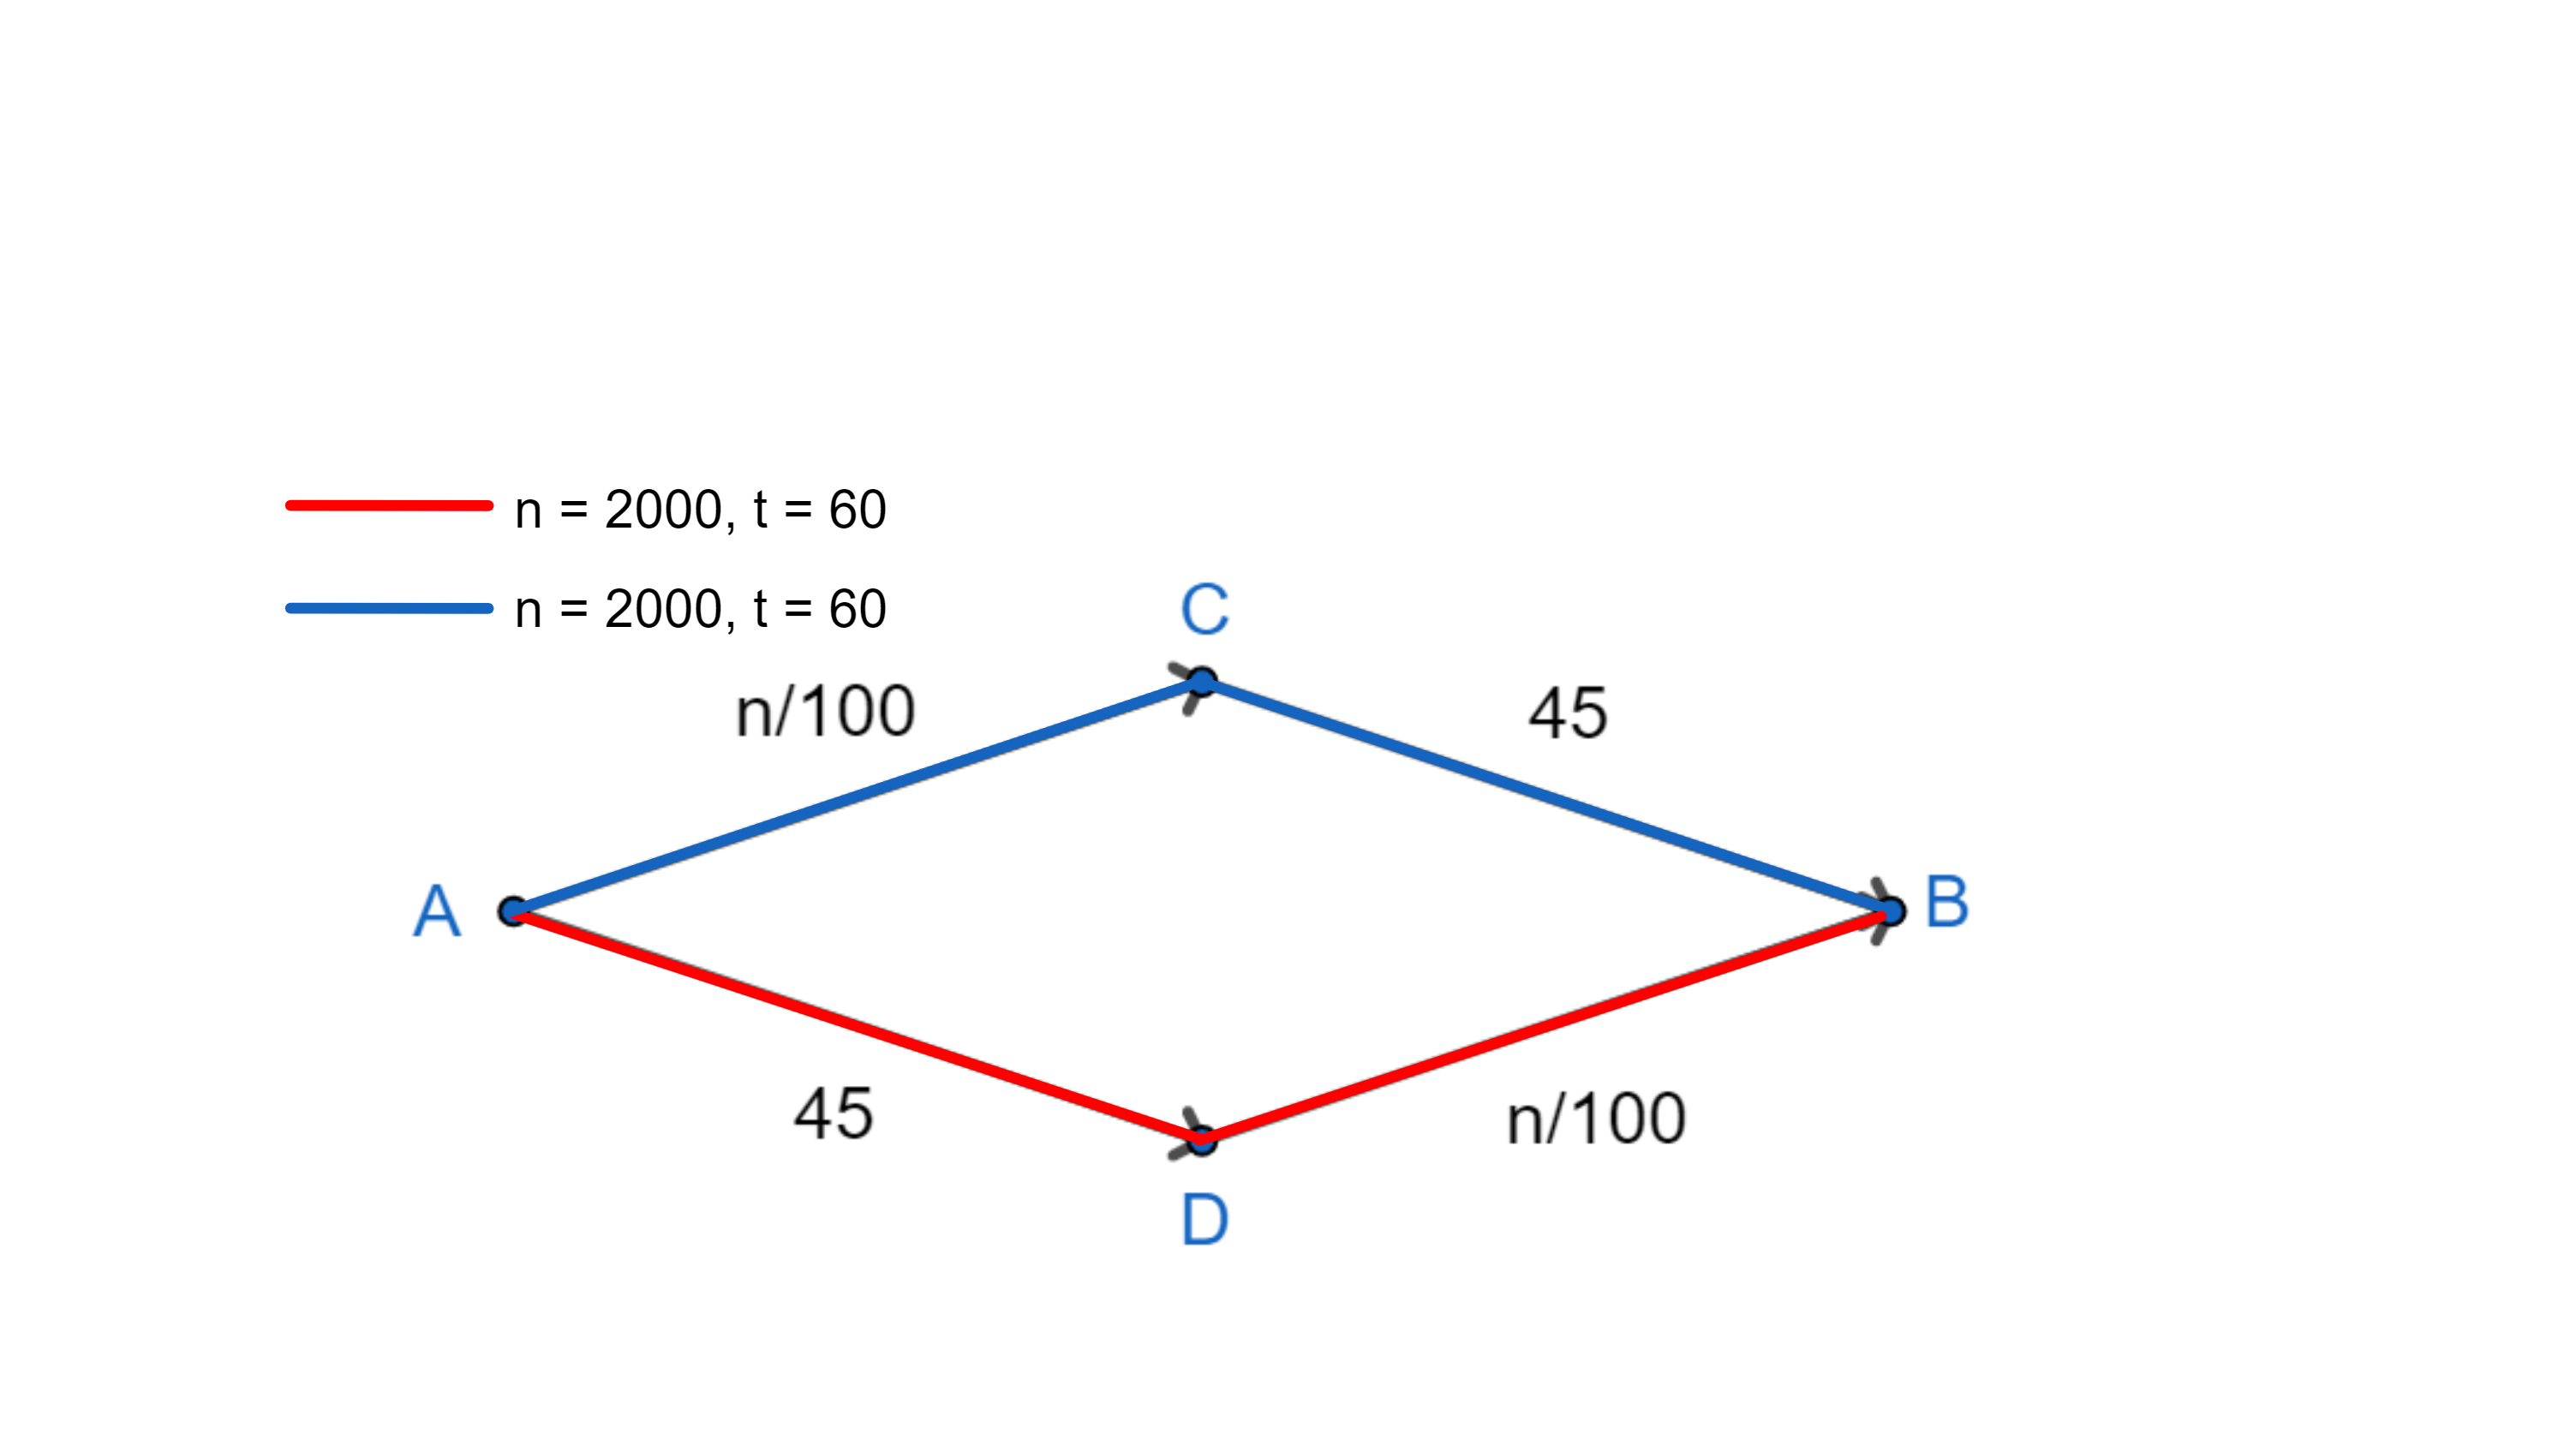
\includegraphics[width=1.1\textwidth, height=60pt]{imgs/before_braess.png}
		\label{ris:braess_1}
			\caption{Оптимальное некооперативное равновесие: $2\,000$ едут по ACB, остальные по ADB. Затраты каждого $\frac{2000}{100} + 45 = 65.$}
	\end{subfigure}
	\hskip 15ex
	\begin{subfigure}[b]{0.3\textwidth}
		\centering
		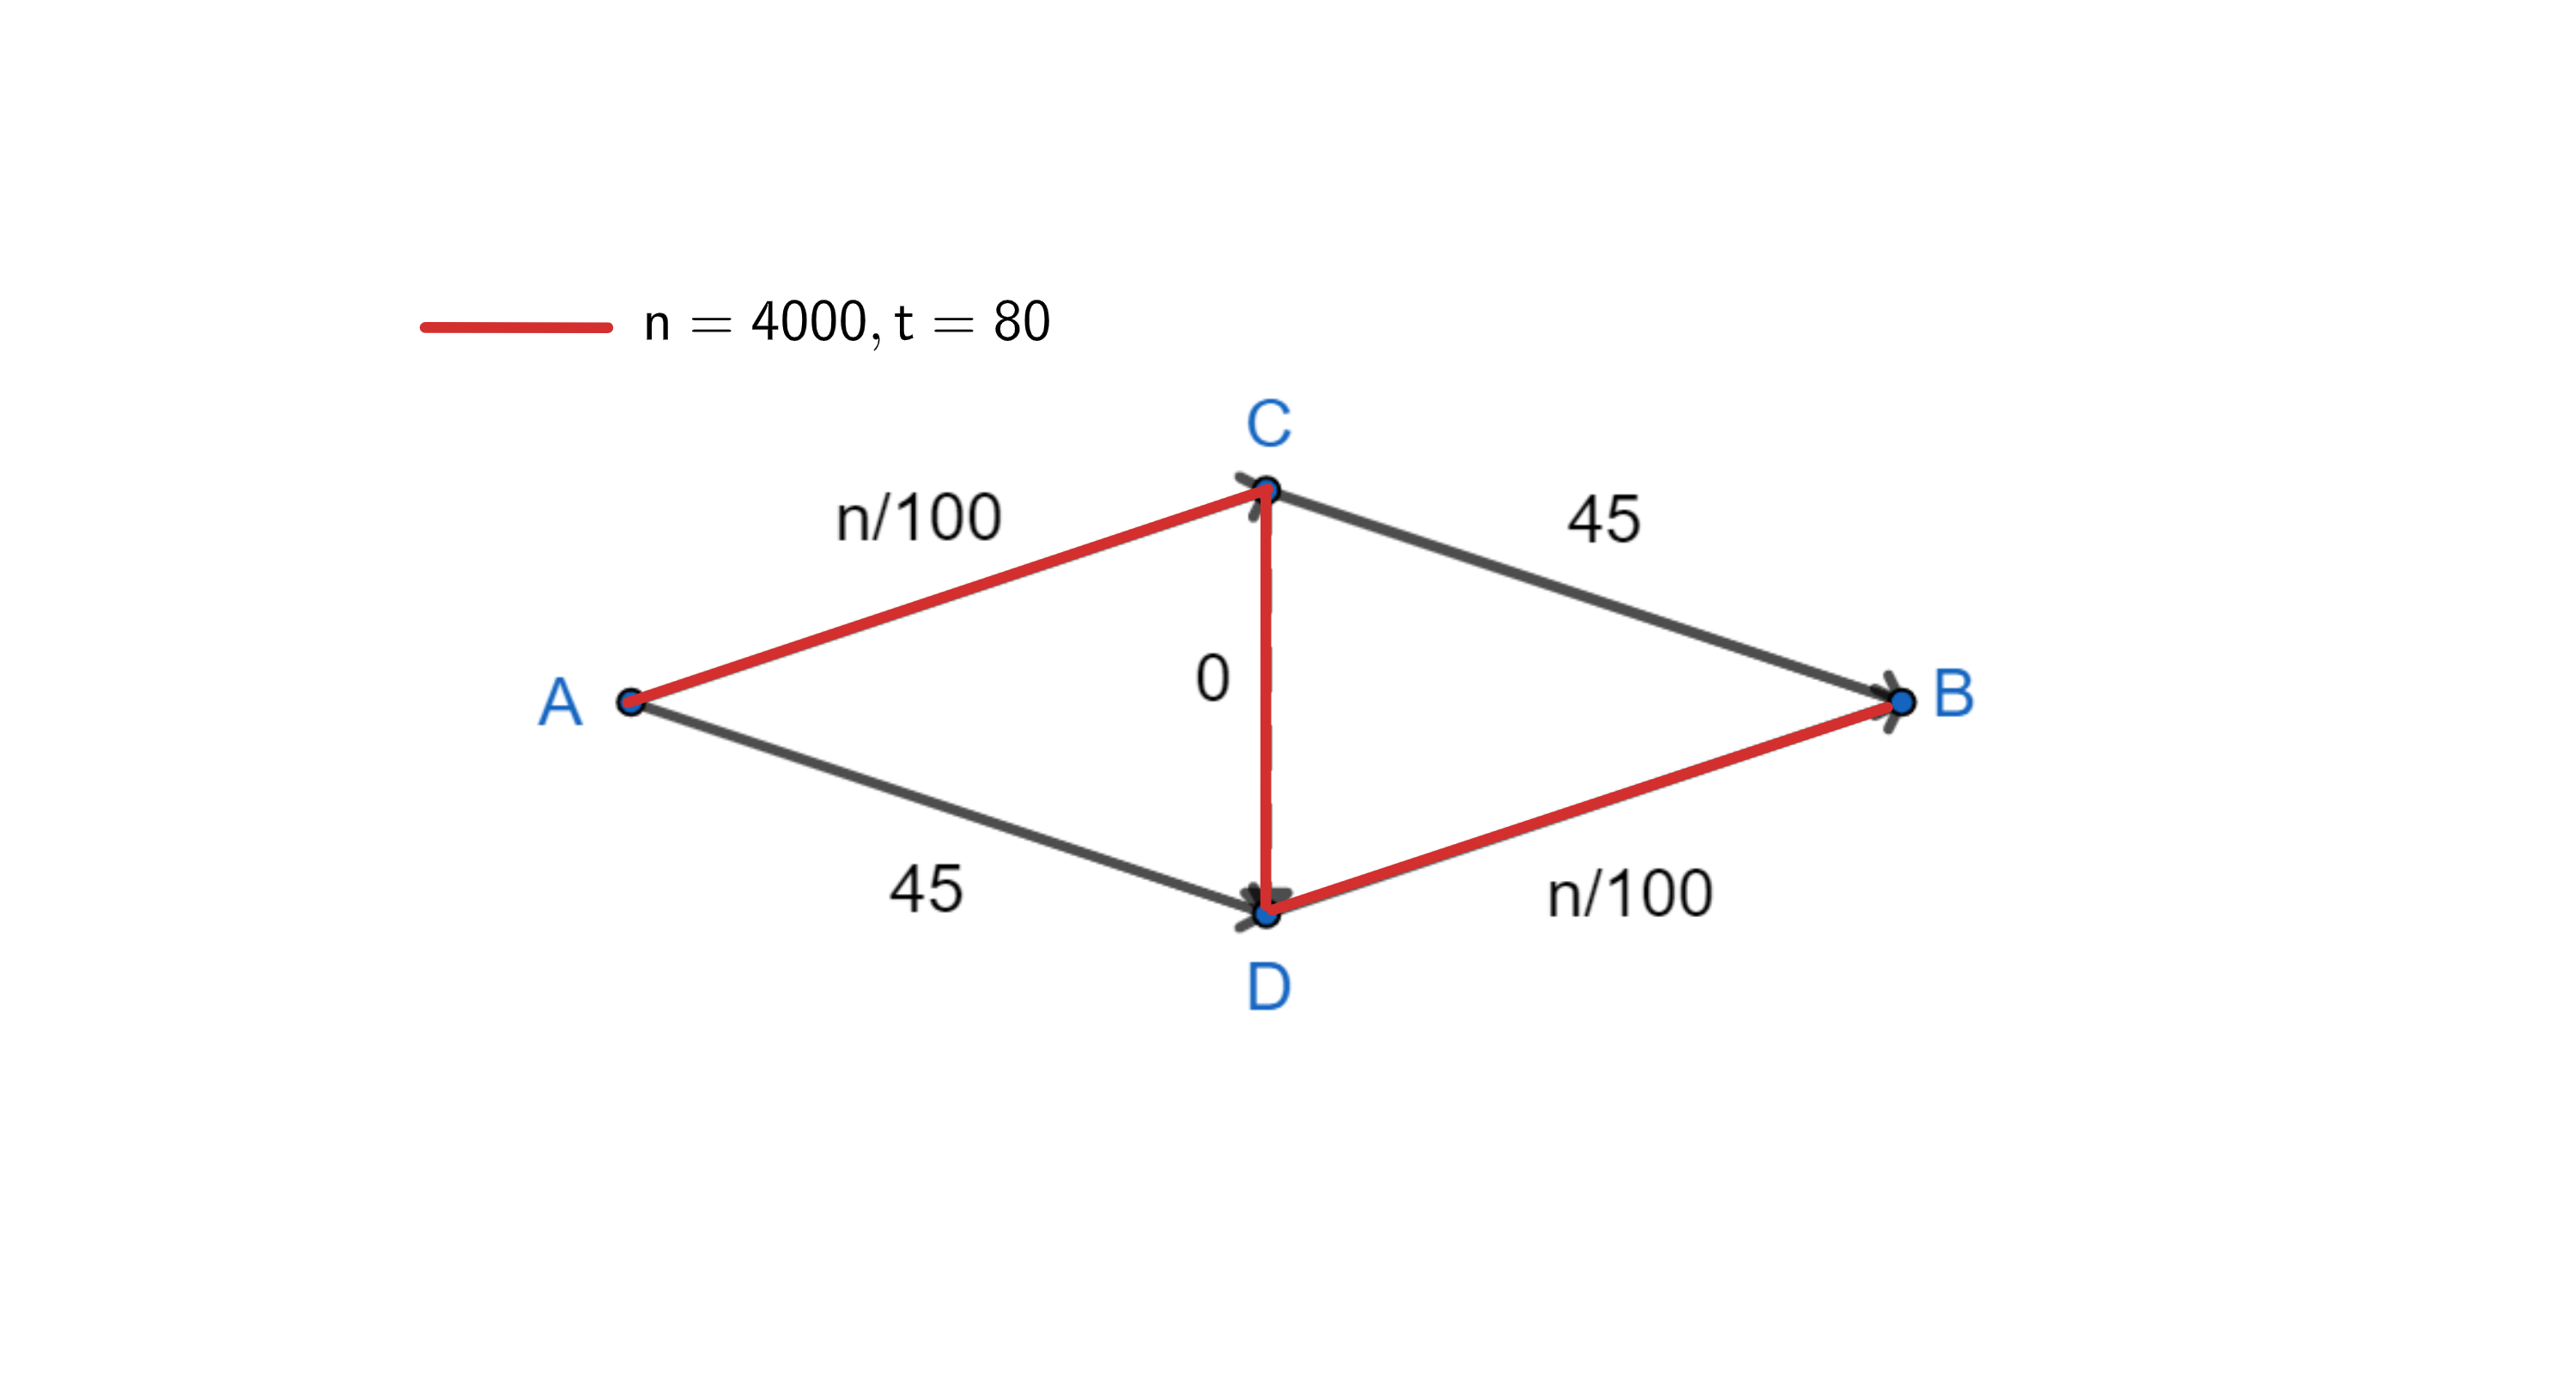
\includegraphics[width=1.1\textwidth, height=60pt]{imgs/after_braess.png}
		\label{ris:braess_2}
			\caption{Добавим ребро CD. Неоптимальное некооперативное равновесие: все едут по ACDB. Затраты: 80.}
	\end{subfigure}
	\caption{Парадокс Браеcа. Метки на ребрах - время проезда $n$ участников по этому ребру. $n = 4000$ участников двигаются из точки $A$ в точку $B$.}
	\label{ris:braess}
\end{figure}

Положим, что временые затраты по ребрам есть 
\begin{align*}
	\overline{\tau}_{AC, i} (\textbf{p}) = &\frac{1}{100}\frac{\int\limits_{0}^{\infty}n_{AC} (\textbf{p}, t)dt}{\int\limits_{n_{AC} (\textbf{p}, t) > 0}dt}, 
	\\
     \overline{\tau}_{CB, i} (\textbf{p}) = &45,
	\\
	\overline{\tau}_{AD, i} (\textbf{p}) = &45, 
	\\ 
	\overline{\tau}_{DB, i} (\textbf{p}) = &\frac{1}{100}\frac{\int\limits_{0}^{\infty}n_{DB} (\textbf{p}, t)dt}{\int\limits_{n_{DB} (\textbf{p}, t) > 0}dt}.
\end{align*}
Предположим, что все участники движения имеют точку отправления $A$ и прибытия $B$. Пусть $n_1 \in \mathbb{Z}_+$ участников выбирают путь $ACB$ и $n_2  \in \mathbb{Z}_+$ участников --- путь $ADB$. Тогда, некооперативное равновесие достигается в случае
$$\frac{n_1}{100} + 45 = \frac{n_2}{100} + 45,$$
то есть $n_1 = n_2$ и временные затраты каждого участника составляют $65$ единиц времени. Такое распределение участников по путям является оптимальным, поскольку является решением задачи оптимизации
$$n_1\left(\frac{n_1}{100} + 45\right) + n_2\left(\frac{n_2}{100} + 45\right) \rightarrow \min\limits_{\substack{n_1 \ge 0, \: n_2 \ge 0 \\ n_1 + n_2 = 4000}}.$$

Теперь добавим в граф ребро $CD$ (см. рис. \ref{ris:braess} \textbf{(b)}) так, что временные затраты на проезд по нему близки к 0:
$$\overline{\tau}_{CD, i} (\textbf{p}) \approx 0.$$
В таком случае никому из участников, передвигающихся через вершину $C$, не выгодно ехать по ребру $CB$. С другой стороны, самый быстрый способ добраться до вершины $D$ --- передвигаться по пути $ACD$. Таким образом, некооперативное равновесие достигается, когда все участники передвигаются по новому пути $ACDB$. При этом они затрачивают $\frac{n}{100} + \frac{n}{100} = 80$ единиц времени. Поскольку стоимость комбинации путей увеличилась, данное некооперативное равновесие перестало быть оптимальным.

Заметим, что для кооперативного равновесия верно обратное:

\begin{state}
Множество кооперативных равновесий $\widetilde{P}$ не пусто, причем
оптимальная комбинация путей является таким равновесием, то есть $\textbf{p}^* \in \widetilde{P}$.
\end{state}

\begin{proof}
	Поскольку для любого $\textbf{p} \in P$ 
	$$\Phi (\textbf{p}^*) \le \Phi (\textbf{p}),$$
	то неравенство верно и для комбинаций путей $$\textbf{p} = \left(p^*_1, \ldots, p^*_{i - 1}, p, p^*_{i + 1}, \ldots, p^*_{n} \right), \text{ } p \in P_i, \text{ } i = 1, \ldots, n.$$
\end{proof}

В некотором смысле кооперативным равновесием можно назвать <<локальный минимум>> функции $\Phi$.

\subsection{Поиск кооперативного равновесия}
Рассмотрим ряд алгоритмов, позволяющих получить некоторое кооперативное равновесие.

Общим свойством всех этих алгоритмов является предположение о том, что существует некоторый алгоритм $\alpha (\Phi_i)$, позволяющий решить задачу оптимизации некоторой функции стоимости $\Phi_i (\textbf{p}) = \phi_i(T_1(\textbf{p}), \ldots, T_n(\textbf{p}))$ посредством выбора пути $p_i$:

\begin{equation}
\label{eq:task_mini}
\alpha (\Phi_i): \Phi_i (\textbf{p}) \rightarrow \min \limits _{p_i \in P_i}
\end{equation}

В работе Л.\,Е.~Разумовой~\cite{Luba} представлен один из таких алгоритмов построения оптимального пути $p_i$ за полиномиальное относительно входных данных время при условии, что функция $\Phi_i (\textbf{p})$ удовлетворяет неравенству
\begin{equation}
	\label{eq:luba_1}
	\Phi_i (p_1, \ldots, p_{i - 1}, pe, p_{i + 1}, \ldots, p_n) \le 
	\Phi_i (p_1, \ldots, p_{i - 1}, qe, p_{i + 1}, \ldots, p_n),
\end{equation}
где $p, \: q$ --- два пути к некоторой вершине $B \in V$, ребро $e$ выходит из этой вершины и путь $p$ <<дешевле>>, чем $q$ относительно стоимости $\Phi_i$:
\begin{equation}
	\label{eq:luba_2}
	\Phi_i (p_1, \ldots, p_{i - 1}, p, p_{i + 1}, \ldots, p_n) \le
  	\Phi_i (p_1, \ldots, p_{i - 1}, q, p_{i + 1}, \ldots, p_n).
\end{equation}

В той же работе показано, что в том случае, когда добавление любого участника не влияет на движение других участников, функции $\Phi_i = T_i$ удовлетворяют условиям  $\eqref{eq:luba_1}, \eqref{eq:luba_2}$ в моделях, описанных в нашей работе. На практике же, это влияние существует. Погрешность алгоритма $\alpha (\Phi_i)$ в таком случае зависит от экстримальных свойств функции $v_i (\textbf{p, t})$.

Предположим, что имеются некоторые функции стоимости $\Phi_i (\textbf{p})$, удовлетворяющие условиям \eqref{eq:luba_1}, \eqref{eq:luba_2}, и процессы оптимизации стоимостей $\phi_i$ и $\phi$ по времени $T_i$ одинаковы:
\begin{equation}
	\label{eq:phi_restr}
	\frac{\partial \phi_i}{\partial T_i} \equiv \frac{\partial \phi}{\partial T_i}, \text{ } i = 1, \ldots, n.
\end{equation}

При условиях \eqref{eq:luba_1}, \eqref{eq:luba_2}, \eqref{eq:phi_restr} возможно описать полиномиальный алгоритм $\beta(\{\Phi_i\}_{i = 1}^n)$, позволяющий перейти к меньшей стоимости передвижения путем изменения некоторого пути  $p_i$ участника $i$. Для поиска кооперативного рановесия достаточно найти неподвижную точку алгоритма $\beta$. 

\begin{algorithm}[H]
	\caption{Поиск неподвижной точки алгоритма $\beta$}
	\label{alg:coop_find1}
	{\bf {Input:}} Начальная комбинация путей $\textbf{p}_0 \in P$, алгоритм $\beta$, количество итераций $iter$\\
	{\bf {Output:}} кооперативное равновесие $\widetilde{\textbf{p}} \in \widetilde{P}$\\
	{\bf {Data:}} $\textbf{p}_{cur}$ - текущая комбинация путей, $\textbf{p}_{new}$ - новая комбинация путей, $i$ - номер итерации
	\begin{algorithmic}[1]
		\State $\textbf{p}_{cur} \gets \textbf{p}_0$
		\State $i \gets 0$
		\While{$i < iter$}
		\State $\textbf{p}_{new} \gets \beta (\textbf{p}_{cur}) $
		\State $i \gets i + 1$
		\If{$\textbf{p}_{new}$ = $\textbf{p}_{cur}$}
			\State \textbf{return $\textbf{p}_{cur}$}
		\EndIf
		\EndWhile
	\State \textbf{return $\textbf{p}_{cur}$}
	\end{algorithmic}
\end{algorithm}

Данный алгоритм не дает гарантий, что сходимость произойдет за число итераций, не зависящее от количества комбинаций путей. Однако результатом каждой итерации алгоритма $\beta$ является новая комбинация путей $\textbf{p}$ меньшей стоимости относительно $\Phi$. 

%Опишем алгоритм, сложность которого не зависит от количества комбинаций путей $|P|$ и, который находит оптимальную комбинацию путей $\textbf{p}$, 
Опишем алгоритм, который с некоторыми допущениями на модель движения имеет полиномиальную сложность и находит оптимальную комбинацию путей $\textbf{p}$.
Также алгоритм не зависит от начальной комбинации путей $\textbf{p}_0 \in P$. Предположим, имеется набор функций $\{\{\Phi_{i, k} \}_{i = 1}^k\}_{k = 1}^n$, для каждого $k$ отображающие декартово прозведение $\prod\limits_{i = 1}^kP_i$ во множество действительных чисел $\mathbb{R}$. Считаем, что все функции удовлетворяют условиям \eqref{eq:luba_1}, \eqref{eq:luba_2}, \eqref{eq:phi_restr}.


\begin{algorithm}[H]
	\caption{Последовательное добавление участников в движение}
	\label{alg:coop_find2}
	{\bf {Input:}} количество участников $n$, алгоритм $\alpha$, алгоритмы $\{\beta_k\}_{k = 1}^n$\\
	{\bf {Output:}} кооперативное равновесие $\widetilde{\textbf{p}} \in \widetilde{P}$\\
	{\bf {Data:}} $\textbf{p}_{k} \in \prod\limits_{i = 1}^kP_i$ - кооперативное отношение для первых $k$ участников, $\textbf{p}_{new}$ - новая комбинация путей, $k$ - номер итерации
	\begin{algorithmic}[1]
		\State $k \gets 0$
		\While{$k <= n$}
		\State $\textbf{p}_{k + 1} \gets (\textbf{p}_{k}, \alpha (\textbf{p}_{k}))$
		\State Запустим алгоритм \ref {alg:coop_find1} на комбинации путей $\textbf{p}_{k + 1}$
		\State $k \gets k + 1$
		\EndWhile
	\end{algorithmic}
\end{algorithm}

При наложенном на модель движения условии, что добавление оптимального пути участника"=эгоиста не меняет свойства оптимальности итоговой комбинации путей, можно сказать, что алгоритм сходится к оптимальной комбинации путей. Для того, чтобы алгоритм сошелся за $n$ применений алгоритма $\alpha$, достаточно изменить условие оптимальности на условие кооперативного равновесия.

%Заметим, что описанные в разделе \ref{sec:models} модели удовлетворяют условиям, описанным выше при функциях стоимости $\Phi_i (\textbf{p}) = T_i (\textbf{p})$.

\newpage
\section{Результаты}

Рассмотрим ряд примеров, которые исследуют экстремальные значения функции затрат задачи $\eqref{eq:target_global_task_T}$, используя подход основанный на поиске <<локального минимума>>. Поскольку данную задачу тяжело промасштабировать на реальные данные, рассмотрим небольшой пример с $n = 30$ участниками на дорожной сети $G$ (см. рис. \ref{ris:graph_average}). Даже в таком небольшом примере существует $8^{30}$ комбинаций путей, перебрать которые не представляется возможным.  Для нетривиальности задачи будем считать, что участники стартуют с небольшими задержками $\Delta t = 0.2$. Иначе, задача сводится к оптимальному распределению масс машин по путям с учетом их взаимодействия. В качестве алгоритма решения задачи \eqref{eq:task_mini} используем обычный перебор путей $p_i \in P_i$. Это решение основано на том, что перебор дает точное решение и требует моделирование всего $|P_i| = 4$ путей, вместо $|E| = 28$ для неточного алгоритма, описанного в \cite{Luba}. 
\begin{figure}[H]
	\begin{center}
		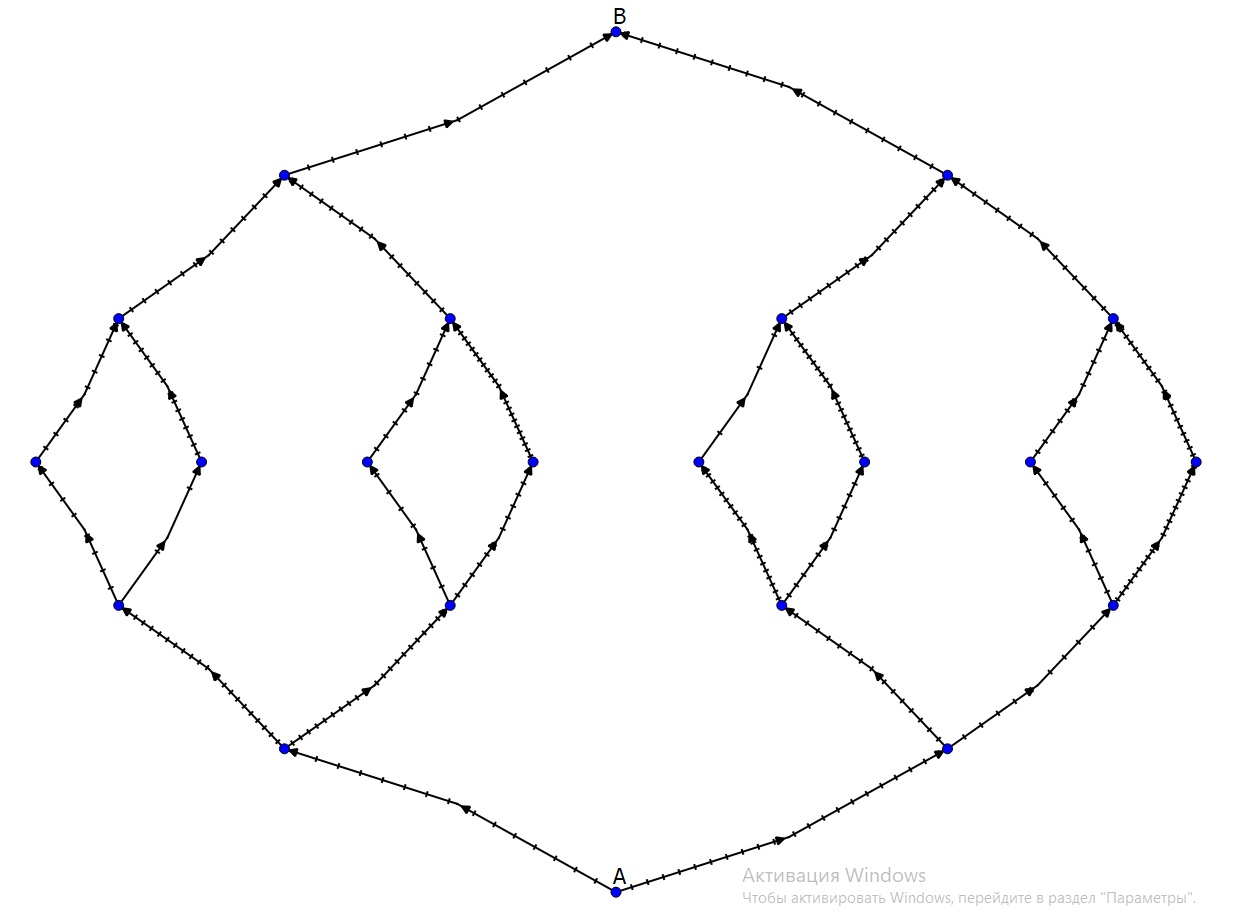
\includegraphics[width = .5\linewidth, height=120pt]{imgs/graph_simple.jpg}
		\caption{Пример дорожной сети. Деление на ребрах - мера длины, равная $L = 500$. $n = 30$ участников передвигается из точки $A$ (нижней) в точку $B$ (верхнюю). }
		\label{ris:graph_average}
	\end{center}
\end{figure}

\subsection{Поиск оптимальной комбинации при одинаковом приоритете участников}

Рассмотрим задачу поиска оптимальных комбинаций путей с функций затрат 
\begin{equation*}
	\phi(T_1, \ldots, T_n) = \sum\limits_{i = 1}^nT_i.
\end{equation*}


Используя эмпирические функции затрат $\overline{\Phi}_i = \Phi$ к задаче \eqref{eq:task_mini}, исследуем алгоритм \ref{alg:coop_find1} на предмет попадания в оптимум. Также для поиска самых невыгодных комбинаций путей можно рассмотреть аналогичную задачу 
\begin{equation}
\label{eq:target_global_task_T_reverse}
\Phi (\textbf{p}) \rightarrow \max \limits_{\textbf{p} \in P}.
\end{equation}
Ожидается, что установив такую цель, участники буду стараться увеличивать общие временные затраты друг друга, используя один и тот же длинный путь. 

Поиск экстремальных значений задач \eqref{eq:target_global_task_T}, \eqref{eq:target_global_task_T_reverse} позволит определить диапазон возможных значений целевой функции $\Phi$. Сравним такие значения со случайным выбором пути, используя равномерное распределение Бернули с $p = 0.5$.

 
\begin{table}[H]
	\caption{Результаты запуска алгоритма \ref{alg:coop_find1}. В таблце представлены значения функции $\Phi$ на полученных комбинациях путей в разных моделях движения с $v_{max} = 60$.}
	\label{tab:res_average}
	\centering
	\begin{tabular}{|c|c|c|c|}
		\hline
		\multicolumn{1}{|c|}{ $\Phi$} & Задача оптимизации    & Модель снижения скорости & Макроскопическая модель \\ \hline
		\multicolumn{1}{|c|}{$T_i$}      & $\Phi (\textbf{p}) \rightarrow \min \limits_{\textbf{p} \in P}$ & 1063.07                  & 5260                    \\ \hline
		\multicolumn{1}{|c|}{$\sum\limits_{i = 1}^n T_i$} & $\Phi (\textbf{p}) \rightarrow \min \limits_{\textbf{p} \in P}$ & 1060.21                  & 5062.5                  \\ \hline
		\multicolumn{1}{|c|}{$T_i$ }      & $\Phi (\textbf{p}) \rightarrow \max \limits_{\textbf{p} \in P}$ & 1576.98                  & 20965.5                 \\ \hline
		\multicolumn{1}{|c|}{ $\sum\limits_{i = 1}^n T_i$} & $\Phi (\textbf{p}) \rightarrow \max \limits_{\textbf{p} \in P}$ & 1576.98                  & 16367.3                 \\ \hline
		\multicolumn{2}{|c|}{ Распределение Бернули ($p = 0.5$)}     & 1185.5                   & 5845.07                 \\ \hline
	\end{tabular}
\end{table}

В таблице \ref{tab:res_average} указаны значения целевой функции в полученных экстремальных значениях $\textbf{p}$. За макроскопическую модель была взята $v_i(\textbf{p}, t) = \frac{v_{max}}{n_e(\textbf{p}, t)}$. Результаты показали, что для модели снижения скорости разница между оптимальным и случайным выбором комбинации путей может составлять более $12\%$, а в худшем случае более $48\%$ (см. рис \ref{fig:average_min_max}). Для макроскопической модели эти значения составляют $15\%$ и $314\%$

\begin{figure}[H]
	\centering
	\begin{subfigure}[b]{0.3\textwidth}
		\centering 
		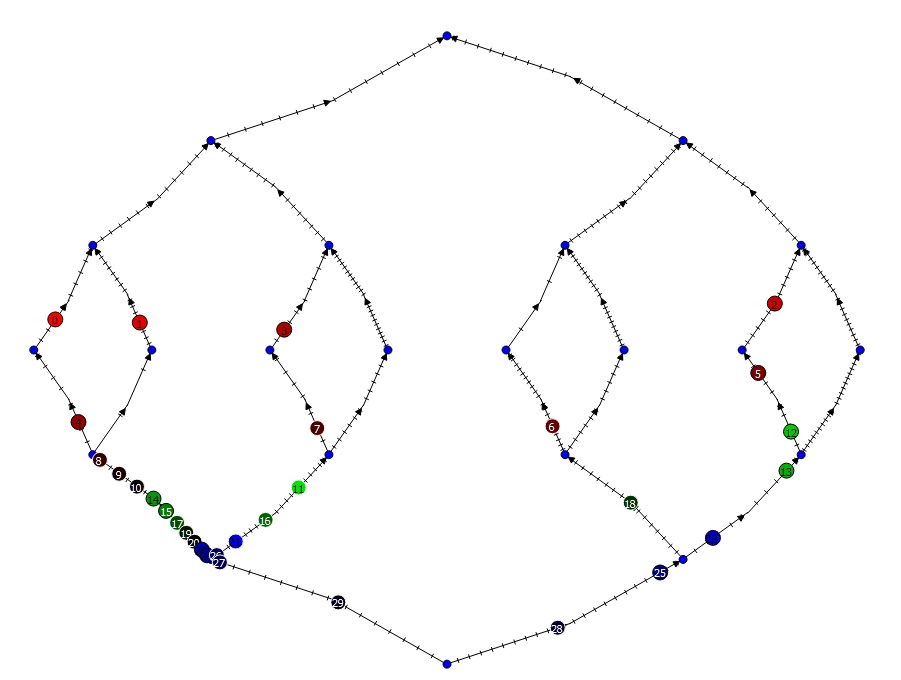
\includegraphics[width=1.1\textwidth, height=60pt]{imgs/average_good.jpg}
	\end{subfigure}
	\hskip 15ex
	\begin{subfigure}[b]{0.3\textwidth}
		\centering
		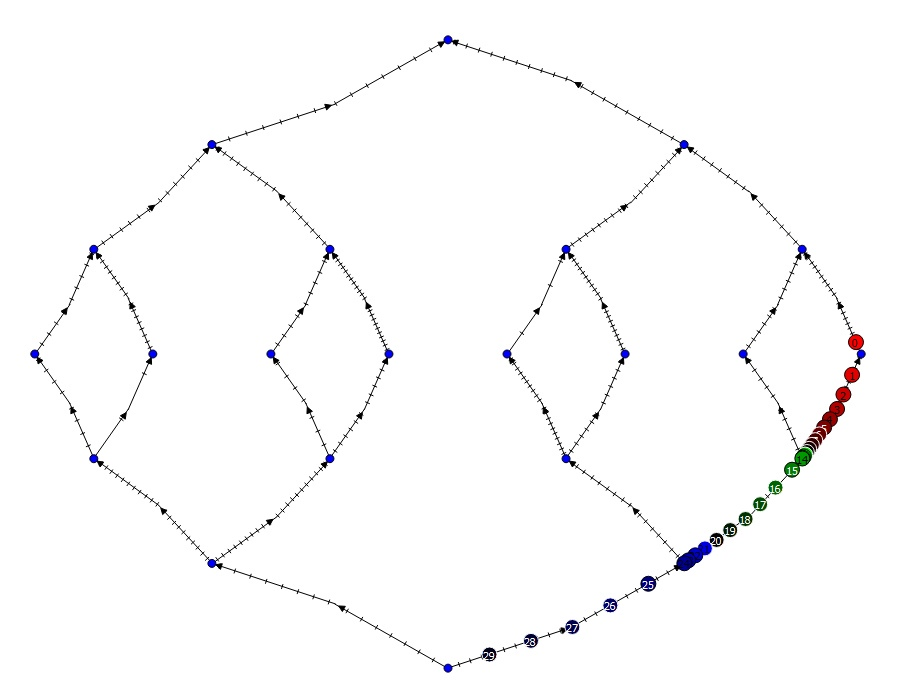
\includegraphics[width=1.1\textwidth, height=60pt]{imgs/average_bad.jpg}
	\end{subfigure}
	\caption{Пример худшего (слева) и лучшего (справа) случая распределения путей участников в модели снижения скорости.}
	\label{fig:average_min_max}
\end{figure}

Такие характеристики позволяют понять как сильно машины могут влиять друг на друга в той или иной модели движения.

\subsection{Поиск оптимальной комбинации с приоритетными участниками}

Рассмотрим задачу поиска оптимальных комбинаций путей с функций затрат 
\begin{equation*}
	\phi(T_1, \ldots, T_n) = \sum\limits_{i = 1}^n h_i T_i,
\end{equation*}
где
$$
h_i =
\begin{cases}
	M \gg 0 ,&  i\text{--- приоритетный участник}, \\
	1 ,&   \text{иначе,} 
\end{cases}
$$

Данная функция затрат описывает ситуацию, когда некоторым участникам необходимо как можно быстрее добраться до своих точек назначения, не повлияв сильно на остальных.

Предположим, что в нашем примере имеется 3 участника с высоким приоритетом. Ожидается, что алгоритм  \ref{alg:coop_find1} сойдется к некоторой комбинации путей, в которой 3 участника занимают, например, левую часть графа, а остальные правую. Оказалось, что в данном случае, качество ответа, выдаваемое алгоритмом \ref{alg:coop_find1} сильно зависит от начальной комбинации путей. Запустив его из случайной комбинации ($p = 0.5$) оказалось, что алгоритм не смог разделить участников на две группы и застрял на некотором некооперативном равновесии (см. рис \ref{fig:prior_good_bad}). 

\begin{figure}[H]
	\centering
	\begin{subfigure}[b]{0.3\textwidth}
		\centering 
		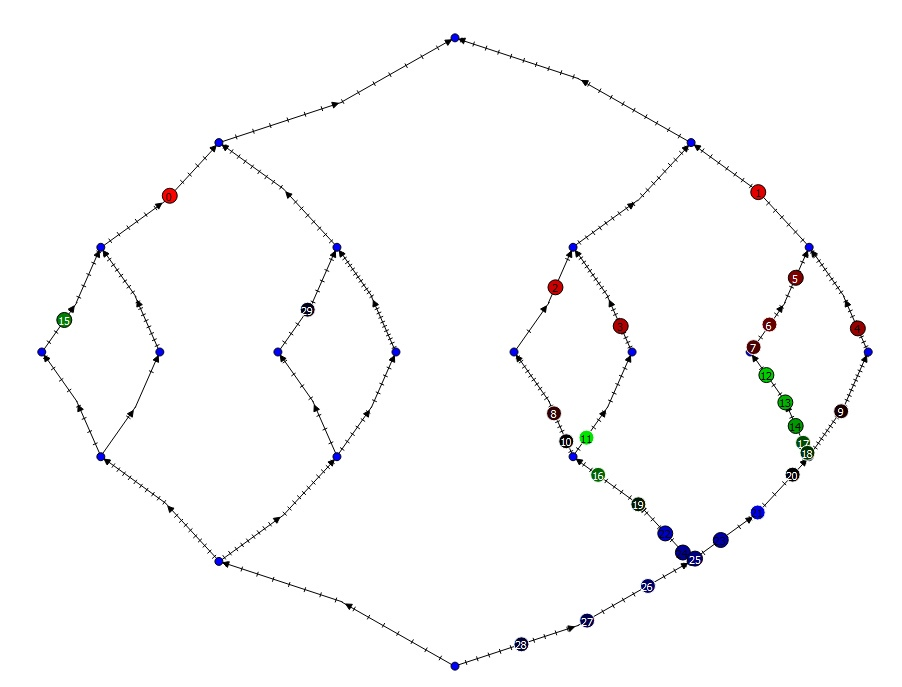
\includegraphics[width=1.1\textwidth, height=60pt]{imgs/prior_good.jpg}
	\end{subfigure}
	\hskip 15ex
	\begin{subfigure}[b]{0.3\textwidth}
		\centering
		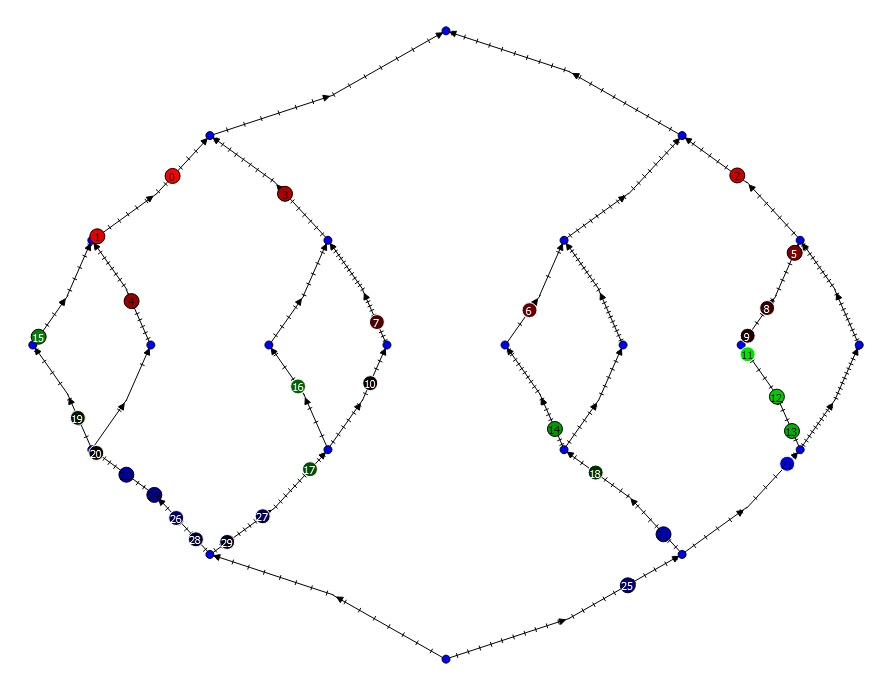
\includegraphics[width=1.1\textwidth, height=60pt]{imgs/prior_bad.jpg}
	\end{subfigure}
	\caption{Оптимальное кооперативное равновесие (слева) с средним временем прибытия $T = 778.34$ и неоптимальное кооперативное равновесие (справа) с средним временем прибытия $T = 950.37$ }
	\label{fig:prior_good_bad}
\end{figure}

\newpage
\section{Заключение}
В работе была поставлена задача поиска оптимальной комбинации путей в терминах произвольной функции временных затрат. Было предложено описание общего принципа взаимодействия участников, заключающегося в задании некоторой модели движения. Мы показали эквивалетность задания функций временных затрат и модели движения.
Для последних была предложена классификация. Среди моделей движения мы выделили класс, для которого доказали возможность сведения задачи поиска оптимальной комбинации путей к задаче смешанного целочисленного линейного программирования. 
Также задача была описана в терминах теории игр, и ее решение было сведено к поиску некоторого равновесия Нэша.
Нами были разработаны алгоритмы нахождения таких равновесий и применены к задачам поиска оптимальной комбинации путей, встречающихся на практике.

    \newpage
\begin{thebibliography}{0}
	
	\addcontentsline{toc}{section}{Литература}
	
	\bibitem{Luba} \textit{Л.\,Е.~Разумова}, ``Построение оптимального маршрута при заданной модели движения других участников движения'' (2022)
	
	\bibitem{book} \textit{А.\,И.~Гасников} ``Введение в математическое моделирование транспортных потоков'' --- Издательство МЦНМО --- 2013. --- 427 с.
	
	\bibitem{min_ip_tsp} \textit{L.~Libralesso} ``Mixed Integer Programming formulations for the balanced Traveling Salesman Problem with a lexicographic objective''. (2020)
	
	\bibitem{braess2} \textit{D.~Braess, A.~Nagurney, T.~Wakolbinger}, ``On a Paradox of Traffic Planning.'' Transportation Science. 39. 446-450. 10.1287/trsc.1050.0127 (2005)
	
	\bibitem{piugou} \textit{A.\,C.~Piugou} ``The economics of welfare'', London: MacMillan, 1932,
	4-th edition. (Русский перевод: Пигу А.С. Экономическая теория благосостояния Т. 1–2, Сер. Экономическая мысль Запада,
	М.: Прогресс, 1985).
	
	\bibitem{teor_igri} \textit{А.\,Г.~Кремлев}, ``Основные понятия теории игр'' --- Екатеринбург : Изд-во Урал. ун-та, --- 2016. --- 144 с
	
	\bibitem{UO} \textit{Ю.\,А.~Олейник, А.\,А.~Зуенко}, ``Глобальные ограничения при моделировании и решении задач в рамках парадигмы constraint programming''. Труды Кольского научного центра РАН. 2020. №8-11.
	
\end{thebibliography} 

\end{document}